% REVISÃO DE LITERATURA--------------------------------------------------------

\chapter{FUNDAMENTAÇÃO TEÓRICA}
\label{chap:fundamentacaoTeorica}

Este capítulo tem como objetivo criar uma fundamentação teórica acerca dos conceitos utilizados na criação da ferramenta proposta neste trabalho. A Seção \ref{sec:engsoft} irá explicar os principais conceitos da Engenharia de Software assim como sua importância no desenvolvimento de uma aplicação. Já a Seção \ref{sec:aplicacoesWeb} discorrerá sobre as especificidades inerentes às chamadas Aplicações Web. Enquanto isso, a Seção \ref{sec:gesinfo} abordará sobre a Gestão da Informação, e como a gestão correta pode impactar nos processos de uma organização. E por último, a Seção \ref{sec:regulamentoaccs} irá descrever sobre o que são as Atividades Curriculares Complementares, e como elas estão presentes na Faculdade de Computação e Engenharia Elétrica.

\section{Engenharia de Software}
\label{sec:engsoft}

A Engenharia de Software, de acordo com \cite{pressman2009engenharia}, engloba processos, métodos e ferramentas que possibilitam a construção de sistemas complexos baseados em computador dentro do prazo e com qualidade, os princípios Engenharia de Software podem ser aplicados em qualquer processo de desenvolvimento de software, sendo que sua utilização aumenta grandemente as chances de sucesso do software desenvolvido. \cite{pressman2009engenharia} explica ainda que o processo da criação de um software engloba cinco atividades estruturais, sendo estas:

\begin{itemize}
    \item Comunicação: antes de se iniciar um projeto, é necessário que haja a comunicação com as partes interessadas para que se saiba quais as suas necessidades;
    \item Planejamento: nesta atividade, é feito um planejamento de como se dará o processo de desenvolvimento de software, quais as estratégias utilizadas e o caminho que deve ser seguido;
    \item Modelagem: os modelos, como descrito por \cite{pressman2009engenharia} podem ser vistos como esboços do projeto que está sendo criado, e tem como objetivo tornar claro o que deverá ser desenvolvido;
    \item Construção: envolve tanto a codificação da aplicação quanto os testes a serem realizados no software.
    \item Emprego: após concluídas as ações anteriores, o software é então entregue às partes interessadas que avaliam o produto e retorna um \textit{feedback} de sua utilização.
\end{itemize}

\cite{pressman2009engenharia} explica que essas ações não precisam ser seguidas à risca, mas que são adaptáveis conforme as necessidades da equipe de desenvolvimento. A Engenharia de Software faz a especificação das atividades apresentadas, separando entre etapas do processo de desenvolvimento de um software.

\subsection{Engenharia de Requisitos}

\cite{elgabry2016requirements} descreve a engenharia de requisitos como sendo o processo de coletar e definir quais serviços serão providos por um sistema de software. A Engenharia de Requisitos serve então para identificar as necessidades das partes interessadas, e transformar essas necessidades em algo que seja útil através de algum tipo de padronização, e então validar os requisitos com as partes interessadas para se determinar se é aquilo que elas realmente precisam.

A primeira ação dentro da Engenharia de Requisitos é a de coleta de requisitos, \cite{pmbok2017} descreve a coleta de requisitos como sendo o processo de determinar, documentar e gerenciar as necessidades das partes interessadas a fim de atingir um objetivo. Quanto mais claros estiverem os requisitos mais simples será a etapa de modelagem e consequentemente maior vai ser a qualidade do produto final em relação à entrega de algo que supra as necessidades das partes interessadas.

Os requisitos de um software estão separados entre funcionais, que conforme descrito por \cite{elgabry2016requirements} se tratam das funcionalidades que um sistema possuirá, e não funcionais, relacionadas aos limites das funcionalidades providas por um sistema, são requisitos como o mínimo de processamento necessário para que o sistema funcione, a resolução mínima que um computador ou celular precisa possuir para acessar o sistema, entre outros.


Dentro do contexto de software voltado para web, \cite{casteleyn2009engineering} descreve os requisitos funcionais como sendo:

\begin{itemize}
    \item Requisitos da Organização: que representa as diferentes visões da organização ou ambiente que uma aplicação será desenvolvida;
    \item Requisitos de Domínio da Aplicação: é aquilo que é necessário que uma aplicação possua de funcionalidades;
    \item Requisitos de Navegação: representa os requisitos necessários para se organizar os diferentes blocos de informação dentro de uma aplicação web;
    \item Requisitos de Interação: refere-se às interfaces com os quais um usuário poderá interagir com a aplicação;
\end{itemize}
	
Os requisitos não funcionais de um software web são classificados por \cite{casteleyn2009engineering} como;

\begin{itemize}
    \item Requisitos do Produto: refere-se ao comportamento da aplicação, como a quantidade de memória necessária para o seu funcionamento, qual a largura de banda de internet mínima necessária, entre outros fatores voltados a arquitetura onde a aplicação funcionará;
    \item Requisitos Organizacionais do Projeto: relacionado a como o projeto está organizado, à forma que equipe de desenvolvimento está estruturada, qual a linguagem de programação utilizada, entre outros fatores organizacionais;
    \item Requisitos Externos: esse requisito está relacionado à fatores externos da organização onde a aplicação está sendo desenvolvida, um exemplo é a capacidade da aplicação estar sempre disponível ao ser hospedada em um site de terceiros, o que não é algo totalmente controlável;
\end{itemize}

\subsection{Modelagem de Requisitos}

\cite{pressman2009engenharia} descreve a modelagem como sendo algo que "abrange tanto análise quanto projeto, descrevendo representações do software que se tornam progressivamente mais detalhadas". Seu objetivo, portanto, é tornar claro o escopo da aplicação, e fazer com que seus requisitos se tornem compreensíveis durante o desenvolvimento da aplicação. Assim, a etapa de modelagem da aplicação tem o objetivo de transformar os dados coletados pela engenharia de requisitos em algo que possa ser entendido e construído pela equipe de desenvolvimento. \cite{casteleyn2009engineering} pontua que nem todos os requisitos precisam ser coletados antes que se dê início à modelagem do software, sendo possível realizar as duas ações de forma paralela.
\cite{pressman2009engenharia}  faz a separação dos modelos de software em quatro tipos:

\begin{itemize}
    \item Modelos baseados em cenários: organiza os requisitos através de cenários que descrevem quais ações os “atores” do sistema terão, e como será o fluxo dessas ações;
    \item Modelos baseados em classes: a modelagem baseada em classes descreve a forma em que os objetos irão estar organizados dentro da aplicação e como esses objetos se comunicam e interagem entre si;
    \item Modelos comportamentais:  este modelo irá indicar o comportamento do software ao receber estímulos ou eventos externos;
    \item Modelos de fluxo: o diagrama de fluxo aborda a forma como os uma visão entrada-processo-saída do sistema, tendo como foco mostrar quais os dados que entram em determinado processo, como esse dado é transformado e qual será a saída resultante do processo;
\end{itemize}

\cite{pressman2009engenharia} divide ainda os modelos em duas visões, a primeira sendo chamada de análise estruturada, e tem como objetivo mostrar como os dados são transformados à medida que são trafegados pelos processos do sistema, já a segunda visão é denominada análise orientada a objetos, e se concentra em indicar quais são as entidades de um sistema e como essas entidades relacionam-se. Apesar de muitas equipes optarem por uma das duas visões excluindo a outra, é possível utilizar ambas se atentando àquilo que agrega valor na modelagem da aplicação.

\section{Aplicações Web}
\label{sec:aplicacoesWeb}

Desde sua criação, a internet tem passado por grandes transformações em sua infraestrutura e na forma como se apresenta àqueles que a acessam, deixando de ser apenas um conjunto de textos e links estáticos e passando a ser composta por aplicações complexas que manipulam grandes quantidades de dados. Tem sido raro encontrar empresas que não utilizam sua infraestrutura seja como forma de divulgação, de prestação se serviços, ou mesmo de gerenciamento de processos. Essa demanda criou uma nova categoria de aplicações, chamadas de \textit{WebApps} ou “Aplicações Web”.

Segundo \cite{casteleyn2009engineering} as aplicações web são normalmente divididas entre uma camada de dados, uma camada de aplicação e uma camada de apresentação. Na camada de dados o desenvolvedor deve entender qual a melhor estrutura para os dados gerados na aplicação, como eles serão relacionados e quais os dados externos à aplicação serão usados. Na camada de aplicação é onde está a maior parte da complexidade do software, ela envolve tanto a implementação da linguagem de programação e da linguagem de marcação utilizada pelo software, como os modelos e protocolos, além de definir a forma como a navegação entre as páginas funcionará. Por último temos a camada de apresentação, onde os desenvolvedores focam seu trabalho no desenvolvimento de interfaces que implementam conceitos de usabilidade e acessibilidade, buscando serem atraentes aos utilizadores.

Há características inerentes à aplicações web que as separam de softwares em geral. Em seu livro, CASTELEYN faz a explanação dessas características:

\begin{itemize}
    \item Alta Acessibilidade de Informação e Serviços: diferente de software desenvolvidos para computadores, as aplicações web devem ser capazes de ser acessadas por qualquer tipo de dispositivo, e diferentes visões e estruturações de informações devem ser feitas de forma a proporcionar essa acessibilidade;
    \item Interface de Hipertexto Centrada no Documento: as informações devem ser mapeadas através da utilização de hipertextos. Há a interação entre diferentes páginas, e deve haver uma preocupação com a forma que o hipertexto é estruturado e exibido ao usuário;
    \item Gerenciamento de Dados, Acesso dos Dados e Tecnologias de Processamento Diferentes: as aplicações web são desenvolvidas com os mais variados tipos de tecnologias, estratégias de tratamento de dados, arquiteturas, entre outros fatores. É necessária uma atenção dos projetistas do sistema em relação às tecnologias que serão utilizadas;
    \item Tecnologias e Motores de Apresentação Diferentes: diferentes formas de apresentação de dados devem ser criadas para que a aplicação possa ser executada em diferentes navegadores e resoluções de tela;
    \item Arquitetura Mais Complexa: a necessidade da adaptabilidade, assim como os diferentes tipos de clientes (navegadores), criam a necessidade de uma arquitetura mais complexa do sistema em relação aos softwares comuns;
\end{itemize}

Durante a etapa de desenvolvimento da aplicação é necessário se estar atento a estas características, elas são fatores importantes que impactam diretamente na aplicação final, e no quão bem a aplicação será capaz de cumprir os requisitos das partes interessadas do sistema.

\subsection{Adaptabilidade}

Uma das maiores características de aplicações web é seu amplo alcance, permitindo que o seu conteúdo seja acessado pelos mais diversos tipos e tamanhos de dispositivos, em diferentes tipos de navegadores e em vários idiomas. Por conta disso, aplicações Web precisam ser adaptáveis e capazes de funcionar em plataformas diferentes. CASTELEYN, faz uma categorização dessas características de adaptabilidade:

\begin{itemize}
    \item Localização e Internacionalização: uma aplicação web pode ser acessada pelos mais diversos grupos de pessoas, das mais variadas localidades, portanto é necessária que haja a inclusão de estratégias de internacionalização dessa aplicação;
    \item Personalização e Adaptabilidade: cada usuário deve ser capaz de ter uma experiência personalizada, ainda que de forma limitada, dentro de um sistema;
    \item Acessibilidade para Usuários com Deficiência: a inclusão de grupos com deficiência tem se tornado exigência no desenvolvimento de software, as aplicações web devem ter isso como principal preocupação levando em consideração o grande número de pessoas que irão acessá-las;
    \item Modelagem para a Adaptação com a Linha de Engenharia do Produto: dadas todas as características já listadas todas envolvem a separação de interesses. Ao identificar esses interesses, é possível separar a aplicação web em determinados segmentos e grupos.
\end{itemize}

Quanto maior for a adaptabilidade de uma aplicação Web, maior o seu alcance. Ao permitir, por exemplo, que pessoas com baixa visão possam utilizar uma aplicação, se inclui uma parcela da sociedade que muitas vezes acaba sendo negligenciada no desenvolvimento de aplicações. Dessa forma, é de grande importância garantir a adaptabilidade dentro do escopo no qual a aplicação se encaixa.


\section{Gestão da Informação}
\label{sec:gesinfo}

Antes de se entender o que é informação, é necessário ter consciência daquilo que a compõe.
\cite{siqueira2005gestao} descreve os dados como uma forma primitiva que compõe um sistema de informação, já a informação é a composição e estruturação desses dados de forma a lhes conceder algum significado. Ela tem se tornado um conceito cada vez mais presente desde a Terceira Revolução Industrial. Segundo \cite{braga2000gestao} "a informação tornou-se uma necessidade para qualquer setor de atividade humana e lhe é indispensável".

O aproveitamento correto das informações deve ser o foco principal de uma organização. Para tanto, surge a Gestão da Informação, que descreve os processos na coleta, transformação e gerenciamento da informação dentro de uma empresa. \cite{braga2000gestao} explica que objetivo da informação é apoiar a política global de uma empresa, tornando mais eficiente o conhecimento e a articulação dos subsistemas que a constituem.

\subsection{Arquitetura e Qualidade dos Dados}

Em seu trabalho, \cite{mcknight2013information} explica sobre a importância da arquitetura de dados dentro de uma organização, segundo o autor "a receita do sucesso começa com uma bem equilibrada e completa abordagem arquitetural". \cite{mcknight2013information} explica ainda que se o dado manipulado por um usuário passa por um processo correto de arquitetura é possível se ter uma análise profunda, perspicaz e rentável do mesmo.


É importante também que haja a garantia de qualidade dos dados gerados dentro de uma organização, pois estes possuem grande impacto em sua sobrevivência. \cite{mcknight2013information}  escreve que qualquer dado em um ecossistema empresarial que é considerado de baixa qualidade será prejudicial para os objetivos do gestor de informações. Essa qualidade dos dados é definida por \cite{mcknight2013information} como sendo a ausência de erros intoleráveis. Em outras palavras, sistemas, assim como os dados que eles manipulam, são passíveis de erro, cabe ao gestor de informação fazer a análise de quais erros são toleráveis ou não dentro de um sistema. \cite{mcknight2013information} indica em seu trabalho fatores em relação à qualidade de dados que devem ser observados:

\begin{itemize}
    \item Integridade Referencial: diz respeito à integridade entre os dados relacionados entre tabelas em um banco de dados, não devem haver referências para dados inexistentes;
    \item Unicidade: cada dado salvo em uma tabela do banco de dados deve possuir um identificador único;
    \item Cardinalidade: restringe a quantidade de referências que podem ser realizadas entre duas entidades;
    \item Subtipo/Supertipo: descreve a hierarquia dos tipos de dados, a forma como as classes de uma aplicação devem ser estruturadas para que façam sentido;
    \item Domínios Razoáveis: utilizado para a análise de dados numéricos;
    \item Múltiplas Colunas de Significado: as colunas de uma tabela dentro de um banco de dados não podem possuir mais de um significado;
    \item Formatação de Erros: os erros devem ser formatados de forma a torná-los mais legíveis;
    \item Dados Opcionais: descreve os dados que são opcionais dentro de uma tabela de banco de dados;
    \item Dados Derivados: são dados derivados de outras aplicações ou bancos de dados;
    \item Dados Completos: é a existência de todos os dados de algum objeto;
    \item Dados Incorretos: é a existência de dados com campos incompletos ou inexistentes;
    \item Codificação dos Dados: descreve o quão limpo é o dado em relação àquilo que a coluna da tabela do banco de dados em que ele está sendo salvo exige.
\end{itemize}

A coleta e organização dos dados como foi vista é essencial em uma empresa, tais dados devem ser estruturados arquiteturalmente de forma que a informação criada por eles possa ser bem aproveitada. Tais princípios devem nortear a construção da solução proposta neste trabalho, de forma que sua implementação vise o melhor aproveitamento dos dados gerados.

\section{Regulamento de ACCs}
\label{sec:regulamentoaccs}

A Secretaria de Educação Superior do Ministério da Educação \cite{min_educ_perguntas} explica que as Atividades Complementares “têm a finalidade de enriquecer o processo de ensino-aprendizagem, privilegiando a complementação da formação social e profissional”. O Parecer CNE/CES 492/2001 realizado por \cite{parecer_492_2001} complementa que “os estágios e atividades complementares fazem parte da necessidade de que haja articulação entre a teoria e a prática, e entre a pesquisa básica e a aplicada”. Dessa forma as atividades complementares visam o enriquecimento da experiência dos alunos, mostrando a prática sobre o que é aprendido. Tais atividades têm seu tempo regulamentado pelo Parecer CNE/CES Nº8/2007 realizado por \cite{parecer_8_2007}, que define um limite máximo de 20\% da carga horária total do curso na Atividade Complementar.

O Parecer CNE/CES 492/2001 realizado por \cite{parecer_492_2001} define ainda algumas atividades autorizadas pelo Colegiado que podem ser usadas como Atividades Complementares:

\begin{itemize}
    \item Estágios;
    \item Iniciação Científica;
    \item Laboratórios;
    \item Trabalhos de Pesquisa;
    \item Trabalho de Conclusão de Curso;
    \item Participação em Eventos Científicos;
    \item Seminários Extra-classe;
    \item Empresa Júnior;
    \item Projetos de Extensão.
\end{itemize}

Tais atividades devem ser realizadas de forma diversificada pelos alunos, limitando a carga horária que pode ser obtida em cada uma delas, esses itens também podem variar conforme as necessidades e particularidades de cada curso.

\subsection{Atividades Complementares na Faculdade de Computação e Engenharia Elétrica}

A Resolução FACEEL - IGE 002/2014 desenvolvida por \cite{faceel2014regulamento} dá o nome de Atividade Curricular Complementar (ACC) às Atividades Complementares, e faz a medição das atividades utilizando pontos, fixando em 61 (sessenta e um) o mínimo necessário para integralização da matéria. A matéria deverá ser feita no 7º semestre no curso de Sistemas de Informação e no 10º nos cursos de Engenharia Elétrica e Engenharia da Computação. O Anexo \ref{anexo:novaResolucaoDeACC} mostra o novo regulamento de ACC que será usado para a integralização de ACCs, como pode ser visto no Anexo as pontuações terão limites, de forma a fazer com que os alunos não foquem em apenas um tipo de ACC, mas que tenham a experiência nas mais variadas áreas.

Na Figura \ref{fig:fluxoAvaliacaoDeACC} é mostrado o fluxo de atividades dentro de uma avaliação de ACC realizada pela coordenação da FACEEL. O discente primeiramente relaciona os seus certificados de ACC aos Tipos de ACC presentes no regulamento \cite{faceel2014regulamento}; após isso, o discente faz o cálculo somatório das pontuações obtidas; O discente então envia os certificados das ACCs por e-mail à coordenação; a coordenação por sua vez verifica os certificados recebidos pelo discente em relação ao regulamento; após isso a coordenação faz a integralização dos pontos obtidos pelo discente no Sistema Integrado de Gestão de Atividades Acadêmicas (SIGAA) da Universidade Federal do Sul e Sudeste do Pará (UNIFESSPA).

\begin{figure}[H]
    \centering
    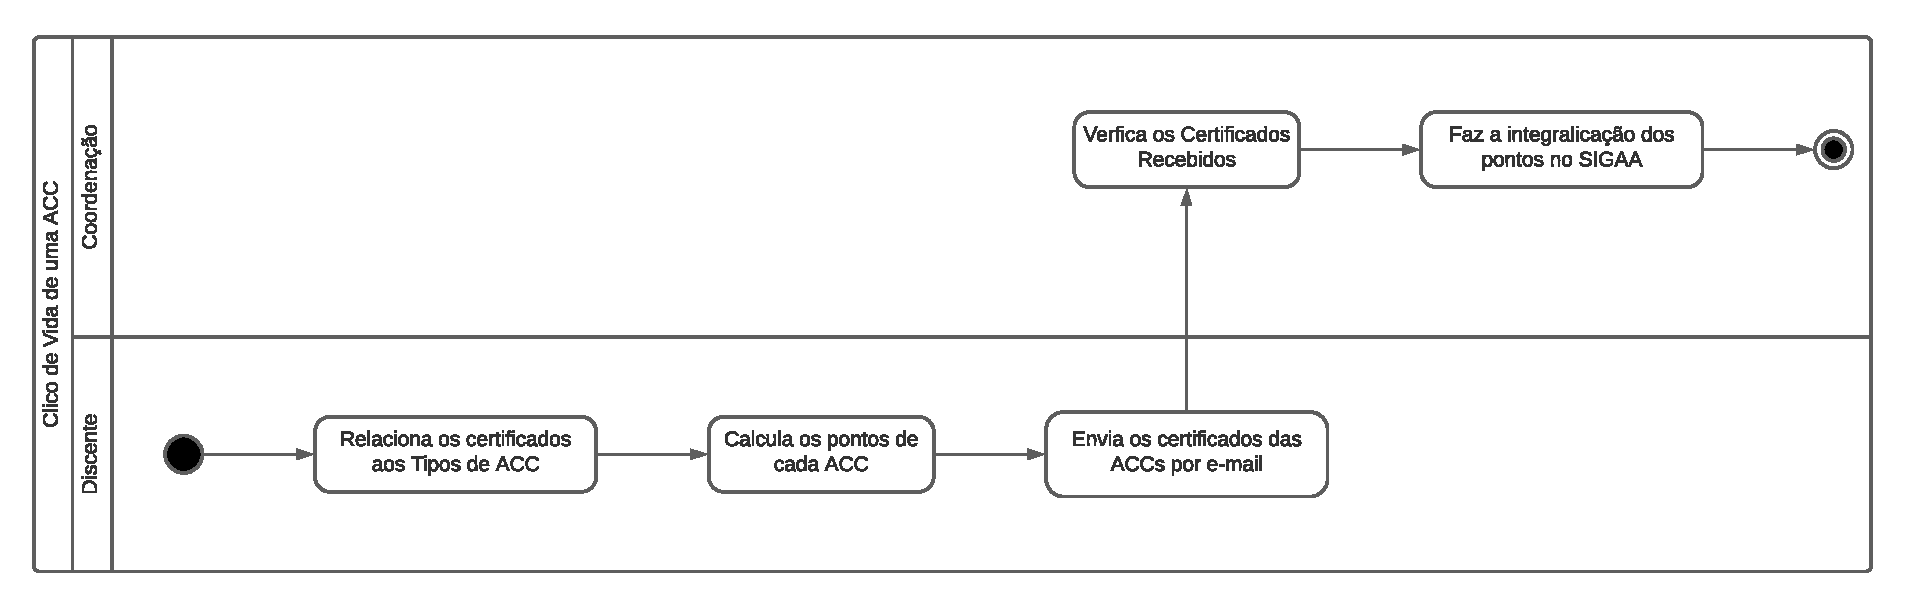
\includegraphics[width=\textwidth]{dados/figuras/Referencial Teórico/avaliacao_acc_manual.pdf}
    \caption{Fluxo de Avaliação de uma ACC}
    \label{fig:fluxoAvaliacaoDeACC}
\end{figure}